% 2010 年辽宁卷文科第 22 题：△ABC 的外接圆，角平分线 AD 的延长线交圆于 E。
% 来源 PDF：普通高考/2010/2010辽宁文.pdf，SHA-256 b402a859318cb9854e9b8257ea128e84f1d52e834556dd80625e883f88dea1fd。
% 原页：第 2 页（A3 三栏）第 2 栏中部，书页码 614。
% 重绘依据：照原页——BC 为接近水平的弦（B 在左、C 在右且略低于 B，弦位略低于圆心），
%   A 在圆上偏左上方，E 在圆上偏下方；AD 与 AE 是同一条直线，D 为它与 BC 的交点；
%   线段 AB、AC、BC、AE、BE 均为实线。
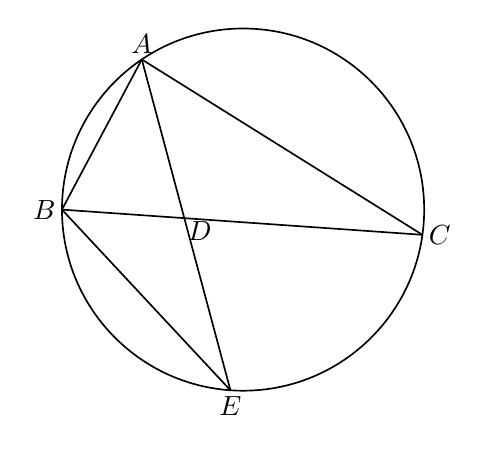
\begin{tikzpicture}[scale=1.15, semithick, line join=round]
  \coordinate (O) at (0,0);
  \coordinate (B) at (180:2);
  \coordinate (C) at (-8:2);
  \coordinate (A) at (124:2);
  \coordinate (E) at (266:2);
  \coordinate (D) at (intersection of A--E and B--C);

  \draw (O) circle[radius=2];

  \draw (A) -- (B);
  \draw (A) -- (C);
  \draw (B) -- (C);
  \draw (A) -- (E);
  \draw (B) -- (E);

  \node[above, inner sep=2pt] at (A) {$A$};
  \node[left, inner sep=2pt] at (B) {$B$};
  \node[right, inner sep=2pt] at (C) {$C$};
  \node[below right, inner sep=1pt] at (D) {$D$};
  \node[below, inner sep=2pt] at (E) {$E$};
\end{tikzpicture}
